% ############################################################################
% DO NOT SUBMIT THIS FILE. IT IS STALE AND CONTAINS KNOWN-WRONG NUMBERS.
%
% paper.tex has since been revised and this file has NOT. Specifically, it still
%   - reports floor_violation_fraction under the "forced assurance loss" label,
%     so its 0.166 baseline and 69.0% headline are the wrong metric
%     (correct: baseline 0.000, headline 67.4%);
%   - presents the two-threshold "law" as a finding when it follows from the
%     link model by substitution;
%   - presents k* = min-cut as a general law rather than an observation;
%   - says one validation check fails when two do;
%   - contains [[Author]] / [[Affiliation]] / [[URL]] placeholders.
%
% Port the revisions from paper.tex before using this as a journal base.
% ############################################################################
%
% EXTENDED VERSION (~7.5 pp). Base for the journal version once updated.
% The 6-page submission variant is paper.tex, which carries the corrected
% results with compressed related work, setup and limitations.
% Compile on Overleaf; not compiled locally (no LaTeX on the authoring machine).
% Figures in ./figures/ as PDF, generated by experiments/make_figures.py and
% experiments/make_fig_architecture.py.
\documentclass[conference]{IEEEtran}
\IEEEoverridecommandlockouts

\usepackage{cite}
\usepackage{amsmath,amssymb}
\usepackage{graphicx}
\usepackage{booktabs}
\usepackage{url}
\usepackage[hidelinks]{hyperref}
\graphicspath{{figures/}}

\newcommand{\GI}{G\textsubscript{1}}
\newcommand{\GII}{G\textsubscript{2}}
\newcommand{\GIII}{G\textsubscript{3}}
\newcommand{\GIV}{G\textsubscript{4}}

\begin{document}

\title{Fail-Closed or Fail-Degraded? Quantifying Forced\\ Assurance Loss in
Contested Multi-Hop QKD Networks}

\author{\IEEEauthorblockN{[[Author]]}
\IEEEauthorblockA{[[Affiliation]]\\ [[email]]}}

\maketitle

\begin{abstract}
In multi-hop trusted-relay quantum key distribution (QKD), secret key is a
depletable per-link resource, since each hop of a relayed path consumes it. How a
network should behave when that key runs short is unsettled. ITU-T Y.3803 permits
degradation, allowing a symmetric cipher to replace one-time-pad key relay, and
field deployments follow it. A parallel line of security engineering refuses,
treating the same transition as a downgrade attack and failing closed instead.
Neither position has been measured against the other. This paper quantifies the
trade-off. We model a nine-node tactical relay formation with per-link key
reservoirs, under an adversary that raises the quantum bit error rate (QBER) until
affected links abort key generation. We introduce \emph{forced assurance
loss}---the fraction of sessions entitled to an information-theoretically secure
key that are served without one---and the \emph{downgrade-forcing cost}, the
adversary budget required to induce it. Suppressing links equal in number to the
minimum edge cut forces the choice. Fail-closed operation then loses availability,
from 0.812 to 0.304. Fail-degraded operation instead preserves availability at
0.973, but serves 69\% of entitled traffic below its authorised grade. The forcing
cost obeys a two-threshold law: the adversary must both exceed a per-link QBER
margin and hold at least the minimum cut; below either threshold its effect is
negligible. A post-quantum fallback removes the sensitivity of availability to
routing policy, but protects only against quantum-channel attacks. These findings
indicate that the assurance-grade composition of served traffic belongs in QKD
resilience reporting alongside key-supply continuity. The simulator, validated
against four published measurements, is released with all configurations.
\end{abstract}

\begin{IEEEkeywords}
Quantum key distribution, trusted-relay networks, key management, post-quantum
cryptography, graceful degradation, military communications.
\end{IEEEkeywords}

\section{Introduction}
A brigade operating in mountainous terrain reaches its rear area through a chain
of relay sites. Command circuits are rekeyed every few minutes, imagery from
forward observation posts is encrypted at one-time-pad rates on the highest-grade
circuits, and logistics traffic is bulk and delay-tolerant. Suppose the network
can no longer supply enough quantum key for all of it. If it refuses service, the
commander sees an outage and responds to it. If instead it keeps the circuit up
but quietly rekeys the imagery link with a computationally secure algorithm
rather than an information-theoretically secure one, the commander sees nothing
at all, and the loss is invisible until someone audits it. Which of those two
failures is preferable is not a settled question, and the two communities that
have addressed it disagree.

The setting that makes the question sharp is the trusted-relay network. Beyond
the reach of a single quantum channel, keys are extended hop by hop: each
intermediate node re-encrypts the end-to-end key under the key it shares with its
neighbour, using a one-time pad and an information-theoretically secure
authenticator~\cite{salvail}. An $n$-hop path therefore consumes key on
\emph{every} one of its $n$ links, and with free-space per-hop rates of order
$10^2$\,bit/s the key supply, not the existence of a quantum channel, is what
binds.

\textbf{The disagreement.} ITU-T Y.3803 cl.~8.2.3~\cite{itu3803} permits
degradation outright: where the keys needed for one-time-pad relay are
unavailable, a symmetric cipher such as AES may be used instead, and the key
manager must record which method it used. Deployments do this~\cite{makris}, and
Tysowski \emph{et al.} put both branches under explicit policy control---on
exhaustion the key manager ``falls back to key derivation if allowed by the
policy, or blocks the host''~\cite{tysowski}. Against this, a recent layered
QKD/post-quantum design treats the same transition as an attack surface,
preventing \emph{downgrade attacks} by tearing down the tunnel after a defined
interval~\cite{spooren}. The worry is older than the mechanism: an adversary who
cannot steal quantum keys will instead deny service precisely in order to
\emph{force} the use of classical cryptography~\cite{schartner}.

\textbf{The gap.} Both positions are architecturally specified and both are
defensible. Neither has been measured. Tysowski \emph{et al.} is a design
document that reports no simulation or experiment, and we are aware of no study
that quantifies what either branch costs, or what an adversary must spend to
force the choice. This matters operationally because the two failure modes are
not merely different in kind: they hand the adversary different currencies.
Refusing converts attack effort into outage, which is visible; degrading converts
it into silent loss of assurance, which is not. Without a measurement, an
operator choosing between them is choosing blind.

\textbf{Contributions.}
(i) A threat-aware degradation model in which adversarial pressure is expressed
in absolute QBER units and a link driven past the security-abort threshold yields
\emph{zero} key, with classical-channel denial and QBER-invisible detector
attacks as distinct states (\S\ref{sec:link}).
(ii) \emph{Forced assurance loss}, a metric defined on traffic \emph{entitled} to
information-theoretic key, and the \emph{downgrade-forcing cost}; we show the
latter obeys a two-threshold law in adversary capability and budget
(\S\ref{sec:head}, \S\ref{sec:sens}).
(iii) Three negative results for key-aware routing once a fallback exists, each
with paired confidence intervals under common random numbers
(\S\ref{sec:routing}).
(iv) A policy-space audit which finds that an interpretable heuristic beats a
searched policy under distribution shift, and explains why (\S\ref{sec:audit}).
(v) A simulator validated against \emph{four} independent published measurements,
one of which it fails---identifying an under-parameterised term in our own key
accounting (\S\ref{sec:valid}).

\section{Related Work}
\begin{table}[t]
\caption{Positioning. \emph{MH} multi-hop trusted relay; \emph{KS} key scarcity;
\emph{PC} priority classes; \emph{CT} contested; \emph{SW} pressure
\emph{swept}; \emph{FB} fallback to weaker crypto; \emph{FA} forced-assurance
metric.}
\label{tab:pos}
\centering\footnotesize
\begin{tabular}{@{}lccccccc@{}}
\toprule
Work & MH & KS & PC & CT & SW & FB & FA\\
\midrule
van Duijn \emph{et al.}~\cite{vanduijn}      & \checkmark & \checkmark & -- & -- & -- & -- & --\\
Mehic \emph{et al.}~\cite{mehic}             & \checkmark & \checkmark & \checkmark & $\circ$ & -- & -- & --\\
Cheng \emph{et al.}~\cite{cheng}             & \checkmark & \checkmark & \checkmark & -- & -- & -- & --\\
Johann \emph{et al.}~\cite{johann}           & \checkmark & \checkmark & -- & -- & -- & -- & --\\
Hao \emph{et al.}~\cite{hao} (RL)            & \checkmark & \checkmark & -- & -- & -- & -- & --\\
Cao \emph{et al.}~\cite{cao} (KoD)           & \checkmark & \checkmark & $\circ$ & -- & -- & -- & --\\
Tysowski \emph{et al.}~\cite{tysowski}       & \checkmark & \checkmark & \checkmark & -- & -- & \checkmark & --\\
Sanz \emph{et al.}~\cite{sanz}               & \checkmark & -- & \checkmark & -- & -- & \checkmark & --\\
Zhu~\cite{zhu}                               & $\circ$ & \checkmark & \checkmark & -- & -- & \checkmark & $\circ$\\
Spooren \emph{et al.}~\cite{spooren}         & \checkmark & -- & -- & $\circ$ & -- & fail-cl. & --\\
Makris \emph{et al.}~\cite{makris}           & \checkmark & $\circ$ & -- & $\circ$ & -- & \checkmark & --\\
Li \emph{et al.}~\cite{li}                   & \checkmark & \checkmark & -- & \checkmark & -- & -- & --\\
Ghorab \emph{et al.}~\cite{ghorab}           & \checkmark & \checkmark & -- & \checkmark & \checkmark & -- & --\\
Hafeez \emph{et al.}~\cite{hafeez}           & \checkmark & \checkmark & -- & \checkmark & \checkmark & \checkmark & --\\
\textbf{This work}                           & \checkmark & \checkmark & \checkmark & \checkmark & \checkmark & \checkmark & \checkmark\\
\bottomrule
\end{tabular}
\end{table}

Table~\ref{tab:pos} positions the work. Two columns matter. \emph{FA} is empty in
every prior row: the fraction of \emph{entitled} traffic forced below ITS key is
not reported anywhere we could find, \cite{zhu} defining the closest antecedent
but neither against swept pressure nor restricted to entitled traffic. And no
prior row combines \emph{FB} with \emph{SW}---works modelling a fallback do not
sweep pressure, and works sweeping pressure do not model a fallback. The
fail-closed/fail-degraded comparison requires both.

Two further strands are close enough to be worth separating from ours. Graded key
delivery already exists: four named assurance levels selected by a central
controller, with a key-derivation function combining a QKD segment and a
post-quantum shared secret at the middle tier~\cite{sanz}; and key-management
architectures place the substitution behind an unchanged delivery interface, so
the consuming application need not know which mechanism served
it~\cite{james}. What none of them reports is what the substitution costs, or how
cheaply an adversary can compel it.

On terminology: in the accepted sense \emph{hybrid} means simultaneous
combination via a key combiner such that the result is secure if at least one
component is unbroken~\cite{ietfhybrid}. A QKD$\rightarrow$PQC substitution is
therefore \emph{not} hybrid, and we call it a labelled grade downgrade. We avoid
``security level'', which already denotes key length in QKD key-management work.

\section{System Model}
\begin{figure*}[t]
\centering
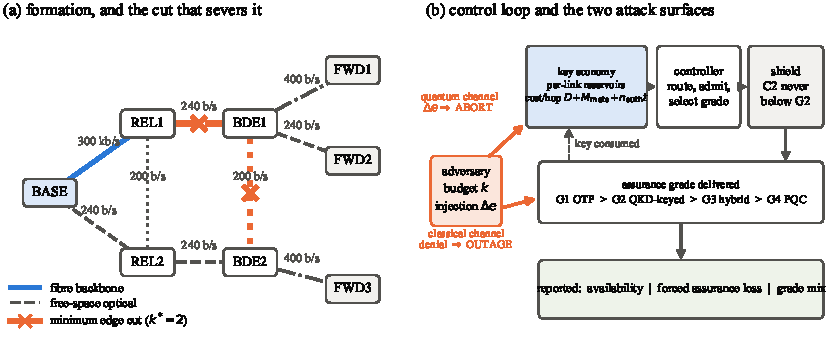
\includegraphics[width=\textwidth]{fig0_architecture.pdf}
\caption{System architecture. (a) The nine-node formation, with per-link secret
key rates and the minimum edge cut marked: suppressing those two links severs
quantum key to two of the three forward posts, which is why $k^*=2$ here.
(b) The control loop. Each session is routed, admitted and assigned an assurance
grade; a hard shield forbids command traffic below \GII; consumption debits the
per-link reservoirs. The adversary has two distinct entry points, and they are not
equivalent---raising QBER on the quantum channel aborts key generation while
leaving the classical channel intact, so the post-quantum grade still works,
whereas denying the classical channel removes that grade as well.}
\label{fig:arch}
\end{figure*}

\subsection{Topology, reservoirs and assurance grades}
We model (T1) a nine-node formation---a rear node, two relays, two brigade nodes,
three forward posts, nine links, one fibre and eight free-space, shown in
Fig.~\ref{fig:arch}(a)---and (T2) a chain of depth $d$ with one longer lateral
alternate. Fig.~\ref{fig:arch}(b) shows where each control decision sits relative
to the key economy.

Reservoirs use the QKDNetSim key-buffer semantics (READY/CHARGING/WARNING/EMPTY
on a threshold and a minimum), and generated key exceeding capacity is
\emph{discarded}. Capacity, threshold and minimum take that simulator's shipped
SECOQC values: $52\,428\,800$, $11\,324\,620$ and $1\,048\,576$ bits. The minimum
doubles as an \emph{authentication reserve}: SECOQC held a 2\,MiB floor purely to
guarantee key for future classical-channel authentication~\cite{peev}. No vendor
publishes a storage capacity, so capacity is swept.

Sessions are served at one of four grades: \GI\ one-time pad (demand $=$ payload
bits, ITS payload, per Shannon~\cite{shannon}); \GII\ QKD-keyed symmetric
(256\,bit, ITS-\emph{delivered} key); \GIII\ hybrid QKD\,$\oplus$\,ML-KEM-768
(128\,bit plus KEM, via an approved domain-separated combiner); \GIV\ ML-KEM-768
only (no quantum key). Each class carries an \emph{authorised floor}. When the
key economy cannot meet it the controller either blocks
(\textsc{fail\_closed}) or serves below it and records an auditable floor
violation (\textsc{fail\_degraded}).

\subsection{Link model and adversary}\label{sec:link}
A two-state model giving a degraded link a fixed fraction of nominal rate is
indefensible under attack: a denial-of-service adversary acts on the quantum
channel specifically to raise noise above the security threshold, and any
perturbation strong enough to do so disrupts key generation
entirely~\cite{alleaume}. We use four states: \textsc{nominal} ($R_0$);
\textsc{degraded} ($R_0\rho(e)$); \textsc{abort} ($0$, for
$e\ge e_{\mathrm{abort}}$); \textsc{outage} ($0$; cut, LOS loss, \emph{or
classical-channel denial}), with
\begin{equation}
\rho(e)=\left[\frac{\max\!\left(0,\,1-fH_2(e)-H_2(e)\right)}
{1-fH_2(e_0)-H_2(e_0)}\right]^{\gamma},
\end{equation}
$f=1.16$ and $e_0=0.03$~\cite{sasaki}. We report $\gamma=1$ (asymptotic BB84
form, following~\cite{ma}) and $\gamma=3.4$, calibrated to the only measured
degraded-link datapoint we found: a deliberately misaligned entanglement link at
QBER 5--7\% delivered 0.25\,kbps against 2--3\,kbps nominal~\cite{sasaki}. These
give 50\% and 10\% at QBER 6\%; \textbf{we publish the disagreement as a
sensitivity rather than resolve it} (\S\ref{sec:sens} shows it barely matters).
$e_{\mathrm{abort}}=0.075$ is an engineering value---the deployed distillation
engine in~\cite{sasaki} provides coding rates only below 3.5, 5.5 and 7.5\%---and
0.11 is reported as a sensitivity. Note that realistic error correction
\emph{lowers} the ITS zero from 11.0\% to 9.9\% at $f=1.16$.

Two failure modes bypass QBER entirely and are separate states, which we state as
a strength: denial of the classical post-processing channel leaves the quantum
channel pristine while halting key production~\cite{mehic}; and detector blinding
by tailored bright illumination makes it possible to ``tracelessly acquire the
full secret key''~\cite{lydersen}, from which it follows that such an attack is
invisible to any QBER-driven model including ours.

The adversary attacks availability to force a downgrade~\cite{schartner}: it
selects $k$ links and injects excess QBER $\Delta e$. Expressing pressure in
absolute QBER units makes it checkable. We report two targeting models, greedy by
edge betweenness and \emph{minimum edge cut}---the honest worst case.

\subsection{Key accounting and traffic}\label{sec:acct}
Relaying $D$ bits of key across one hop costs
$D+M_{\mathrm{meta}}+n_{\mathrm{auth}}t$, with metadata 240\,bit (Y.3803 relays a
\emph{key file}, not a bare key) and authentication tag $t=127$\,bit~\cite{walenta}.
Wegman--Carter authentication is charged per message and grows only
\emph{logarithmically} in message length~\cite{fung}, so the overhead is a
function of block size: at $D=256$ the total is 2.93 times the delivered key, and
at $D=1$\,Mbit it is 1.000. Setting the authentication terms to zero recovers the
bare $D{\cdot}n$ law used throughout the routing literature, which we treat as an
ablation.

The count $n_{\mathrm{auth}}$ of authenticated messages per key delivery is the
one term we could not ground in a specification. We initially set it to 2, from
the observation that mutual authentication consumes two independent one-time keys
per round. \S\ref{sec:valid} shows this is a lower bound rather than a
measurement: published relay overhead implies $\approx7$ and an application-level
tunnel $\approx40$. We therefore report it as a swept parameter and re-check the
headline across the range.

Demands come from measured deployments. C2: 2048\,bit, floor \GII, 5\,s,
$\lambda=0.05$\,s$^{-1}$ (256\,bit/min per encryptor is the modal deployed
unit~\cite{stucki}). ISR: 144\,000\,bit, floor \GI, 30\,s,
$\lambda=0.02$\,s$^{-1}$---a 60\,s session of the 2.4\,kbps real one-time-pad
voice run for 31 months on a 46-node metropolitan QKD network~\cite{chen}. LOG:
320\,000\,bit, floor \GIII, 120\,s, $\lambda=0.03$\,s$^{-1}$, from the same
network's measured 320\,kbps file transfer.

\section{Experimental Setup}\label{sec:setup}
Discrete-event simulation at 1\,s resolution, 24\,h horizon with the first 12\,h
discarded. The warm-up is itself a finding: with reservoirs initialised full,
free-space stores take $\sim$12\,h to fall to the authentication reserve, and
half-run metrics agree only thereafter. A 4\,h run leaves them at 59\% of
capacity and measures the initial fill, not the key economy.

Policies use \emph{common random numbers}---identical arrival streams and channel
realisations per seed---so comparisons are paired; intervals are paired
bootstraps (20\,000 resamples). Twelve seeds for the main comparisons, six for
sweeps.

\subsection{Why a purpose-built simulator}
Cross-validating against an established quantum-network simulator would be the
natural check, and we could not do it, for a reason worth stating precisely
rather than glossing. Source-tree inspection shows that SeQUeNCe implements
point-to-point BB84 with Cascade reconciliation and has no trusted-relay or
key-pool model; QuISP models entanglement distribution and has no key pools; and
NetSquid has neither, while additionally distributing both package and
documentation behind registration under a non-OSI licence, which is an
artifact-availability problem for a reproducible paper. \emph{A key-economy
simulator cannot be validated against tools that do not model a key economy.}

QKDNetSim is the sole on-target candidate, and we adopt its key-buffer semantics
verbatim---the four buffer states and the overflow-discard rule---so that our
reservoir is a citable object rather than an invention. We did not cross-validate
against it. Its routing is self-described as an early implementation, its
controller offers a single policy, and \emph{admission control is absent}, which
is one of the two mechanisms this paper compares; and QKDNetSim+ reports that
nodes there did not adequately process received key material and that the crypto
handler malfunctioned~\cite{qkdnetsimplus}---defects in precisely the layer a
cross-validation would exercise. Validating against a tool with known faults in
the layer under test is not obviously an improvement. We list it as future work.

\subsection{Validation against four published measurements}\label{sec:valid}
Instead we constrain the model from four independent directions, using
measurements from three deployments. A 43-check gate covering key conservation,
reservoir bounds and state transitions, the rate cliff and the degenerate cases
in both fail modes must pass before any result is reported; on top of that we
reproduce the following.

\begin{table}[t]
\caption{Validation against published measurements. Two checks disagree, in the
same direction, and the disagreement identifies an under-parameterised term.}
\label{tab:valid}
\centering\footnotesize
\begin{tabular}{@{}llll@{}}
\toprule
& Quantity & Measured & Model\\
\midrule
V1 & key-store drain~\cite{peev} & 3584\,s & \textbf{3584\,s}\\
V2 & relay overhead~\cite{dynes} & 3.69$\times D$ & 2.23$\times D$\\
V3 & auth.\ share~\cite{peev} & 91.2\% & 65.9\%\\
V4 & OTP voice pairs~\cite{chen} & 11 & 1.2--12.6\\
\bottomrule
\end{tabular}
\end{table}

\textbf{V1} reproduces the SECOQC rerouting experiment, in which an
8192\,bit/s one-time-pad application drained 3.5\,MiB of a 5.5\,MiB key store in
approximately one hour: we obtain 3584\,s against a reference of 3584\,s.
\textbf{V4} is a capacity check on the one-time-pad demand law and passes without
tuning---eleven simultaneous bidirectional 2.4\,kbps voice pairs require
52.8\,kbps, inside the 6--60.5\,kbps range measured on that network.

\textbf{V2 and V3 both fail, and they fail the same way.} Cambridge distributed
1000 global keys at a cost of about 180\,kbyte of link key, i.e.\ 3.69 times the
$\sim$400-bit key delivered, where our accounting predicts 2.23. SECOQC's
AES-encrypted tunnel consumed 5824\,bit per rekey round of which only 512\,bit
was cipher key---91.2\% authentication---where we predict 65.9\%. Solving each
measurement for the number of authenticated messages per key delivery gives
$n_{\rm auth}\approx7$ for a relay hop and $\approx40$ for an application-level
tunnel, against the value 2 we had assumed from the mutual-authentication
argument. \textbf{Our $n_{\rm auth}=2$ is a lower bound, not a measurement, and
our per-hop key cost is correspondingly optimistic.}

We treat this as a result rather than an embarrassment, for three reasons. It
fixes the \emph{direction} of our bias, which is what a reader needs in order to
use the numbers. It strengthens the accounting finding of
\S\ref{sec:acct}---calibrated to Cambridge, the understatement in the
literature's bare $D{\cdot}n$ law grows from 2.93$\times$ to 5.41$\times$ for
256-bit blocks. And it forced a re-check of the headline at the calibrated value,
reported in \S\ref{sec:sens}, which the headline survives.

\section{Results}
\subsection{The fail-closed/fail-degraded exchange rate}\label{sec:head}
\begin{figure*}[t]
\centering
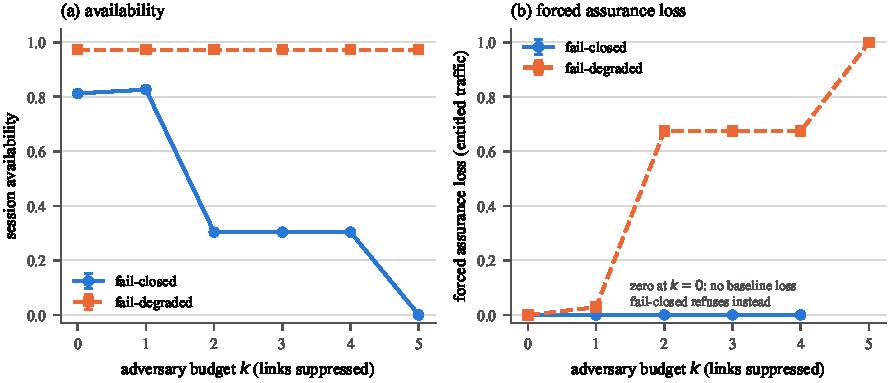
\includegraphics[width=\textwidth]{fig1_failmode.pdf}
\caption{Availability (a) and forced assurance loss (b) versus adversary budget
$k$, for fail-closed and fail-degraded operation. Error bars: SD over 12 seeds.
Fail-closed cannot lose assurance by construction---it refuses instead.}
\label{fig:failmode}
\end{figure*}

\begin{table}[t]
\caption{Availability and forced assurance loss versus adversary budget
(12 seeds, key-aware routing, $\Delta e=0.05$, betweenness targeting).}
\label{tab:head}
\centering\footnotesize
\begin{tabular}{@{}llrrrrr@{}}
\toprule
Mode & $k$ & Avail. & Blocked & \GII & \GIV & Forced\\
\midrule
\textsc{closed} & 0 & 0.8124 & 0.1876 & 0.590 & 0.000 & \textbf{0.000}\\
\textsc{closed} & 1 & 0.8264 & 0.1736 & 0.564 & 0.000 & \textbf{0.000}\\
\textsc{closed} & 2 & \textbf{0.3039} & 0.6961 & 0.508 & 0.000 & \textbf{0.000}\\
\textsc{closed} & 5 & \textbf{0.0000} & 1.0000 & --- & --- & ---\\
\textsc{degr.}  & 0 & 0.9733 & 0.0267 & 0.659 & 0.000 & 0.166\\
\textsc{degr.}  & 1 & 0.9733 & 0.0267 & 0.607 & 0.029 & 0.157\\
\textsc{degr.}  & 2 & 0.9733 & 0.0267 & 0.174 & \textbf{0.675} & \textbf{0.690}\\
\textsc{degr.}  & 5 & 0.9733 & 0.0267 & 0.000 & \textbf{1.000} & \textbf{1.000}\\
\bottomrule
\end{tabular}
\end{table}

The transition is a cliff (Table~\ref{tab:head}, Fig.~\ref{fig:failmode}).
Suppressing 2 of 9 links collapses fail-closed availability from 0.812 to 0.304,
while fail-degraded operation holds availability at 0.973 and converts the same
pressure into 69.0\% forced assurance loss, post-quantum-only service rising from
2.9\% to 67.5\%. At $k=5$ both endpoints are total: complete denial, or complete
assurance loss at undiminished availability.

\textbf{The general law, not the instance.} The value 2 is a property of the cut
structure, not of our formation: $k^\ast$ equals the \emph{minimum edge cut}
separating the rear node from the forward posts. Here two links are the only
quantum-viable route into one brigade node, so the cut is 2 and availability
floors at one third. \S\ref{sec:cost} confirms the law on a chain where the cut is
2 at \emph{every} depth.

\textbf{The authorised policy is infeasible even unattacked, and we say so.} At
$k=0$, 16.6\% of entitled traffic is already forced below its floor: at the
free-space rates cited, a one-time-pad floor for a 144\,kbit session is not
fundable. Either the rate must rise or the floor must relax to periodic symmetric
rekeying.

\subsection{Three negative results for key-aware routing}\label{sec:routing}
\begin{table*}[t]
\caption{Policy comparison, paired bootstrap over common seeds (20\,000
resamples, 12 seeds), $k=0$. SP: shortest path. KAR: key-aware. CAF: class-aware
floors. Set full width because the paired intervals are the result---reporting
them only in prose would leave a reader unable to see that the fail-degraded
differences are exactly zero while KAR's fail-closed deficit is not.}
\label{tab:policy}
\centering\footnotesize
\begin{tabular}{@{}llrrrr@{}}
\toprule
Mode & Policy & Avail. & $\Delta$ vs SP [95\% CI] & Forced & Key (Mbit)\\
\midrule
\textsc{degr.} & SP      & 0.9733 & reference & 0.166 & 436.8\\
\textsc{degr.} & KAR     & 0.9733 & $+0.0000\ [0.0000,0.0000]$ & 0.157 & 463.7\\
\textsc{degr.} & KAR+CAF & 0.9733 & $+0.0000\ [0.0000,0.0000]$ & 0.166 & 398.7\\
\midrule
\textsc{closed} & SP      & \textbf{0.8392} & reference & 0.3569 & 437.8\\
\textsc{closed} & KAR     & \textbf{0.8124} & $\mathbf{-0.0268\ [-0.0293,-0.0243]}$ & 0.3687 & 464.1\\
\textsc{closed} & KAR+CAF & \textbf{0.5092} & $\mathbf{-0.3299\ [-0.3333,-0.3264]}$ & \textbf{0.0000} & 399.3\\
\bottomrule
\end{tabular}
\begin{flushleft}\footnotesize
Under fail-degraded operation the three policies coincide on availability
\emph{exactly}: the confidence interval has zero width because the post-quantum
fallback succeeds on every session for which a classical path exists, in every
seed. Mean path length is 3.060--3.128 hops throughout and is omitted for space.
\end{flushleft}
\end{table*}

\textbf{(1) The service metric becomes degenerate.} Under fail-degraded operation
the paired availability difference between all three policies is $0.0000$ with a
95\% CI of \emph{zero width}, because the fallback succeeds wherever a classical
path exists. Availability is then a property of connectivity, not of
key-awareness: \emph{the metric the key-aware-routing literature reports stops
responding to the thing it measures}. Routing still moves key expenditure
significantly (KAR $+27.0$\,Mbit, CI $[+25.3,+28.9]$; floors $-38.1$\,Mbit, CI
$[-40.5,-35.7]$).

\textbf{(2) Key-aware routing is worse.} Under fail-closed operation KAR loses
2.7 points of availability to shortest path ($-0.0268$, CI
$[-0.0293,-0.0243]$). The mechanism is the hop multiplier: KAR selects marginally
longer paths (3.086 vs 3.062 hops) and every extra hop consumes key on an
\emph{additional} link, raising expenditure 6.0\% and starving later sessions.
Sweeping the hop penalty over four orders of magnitude does not repair it: at
penalty $10^3$ KAR converges to shortest-path behaviour (3.065 hops,
440.0\,Mbit) rather than beating it. We scope the claim to its three joint
conditions---binding scarcity at steady state, fail-closed semantics, and a
hop-multiplied cost with authentication charged. Where prior work reports 25--40\%
improvements~\cite{cvitic} it measures blocking under different scarcity and
without a fallback.

\textbf{(3) Reservation floors are a Pareto trade.} Class-aware floors convert
availability into assurance: $0.839\rightarrow0.509$ in exchange for forced loss
$0.357\rightarrow0.0000$. Every session served carries an ITS-delivered key.

\subsection{Downgrade-forcing cost versus depth}\label{sec:cost}
\begin{figure}[t]
\centering
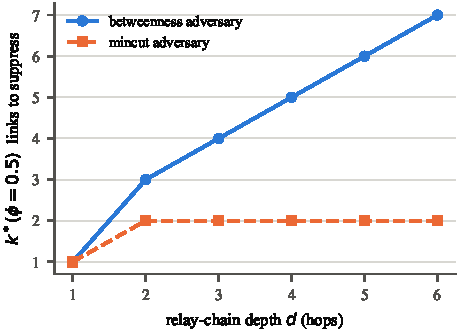
\includegraphics[width=\columnwidth]{fig3_forcing_cost.pdf}
\caption{Downgrade-forcing cost $k^\ast(\phi{=}0.5)$ versus relay-chain depth for
a greedy centrality-guided and an optimal minimum-cut adversary.}
\label{fig:cost}
\end{figure}

Measured on \emph{forced} degradation (nominal loss is 0.000 at every depth, so
every point is attributable to the attack), a greedy centrality-guided adversary
requires $k^\ast=d+1$, growing linearly with depth, because it exhausts the
already-severed primary path before touching the alternate. A minimum-cut
adversary requires \textbf{exactly two links at every depth}
(Fig.~\ref{fig:cost}). At $d=6$ that is a $3.5\times$ overstatement of resilience
if only the greedy adversary is reported. \emph{Adding relay depth buys no
protection against a competent adversary.}

\subsection{Sensitivity and the two-threshold law}\label{sec:sens}
\begin{figure*}[t]
\centering
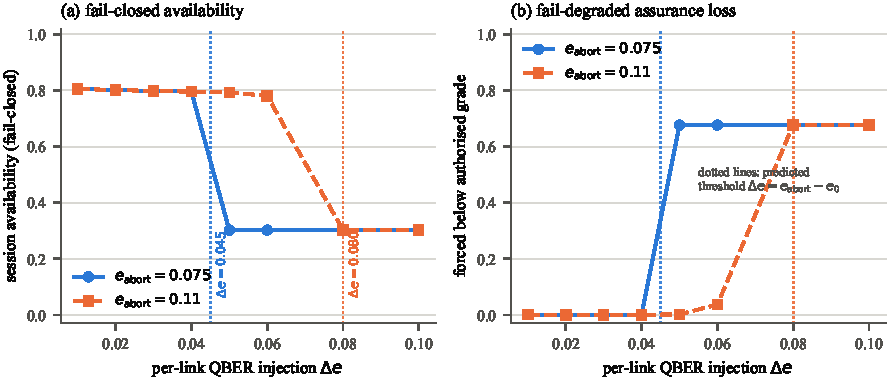
\includegraphics[width=\textwidth]{fig7_two_threshold.pdf}
\caption{The two-threshold law. Dotted vertical lines mark the \emph{predicted}
capability threshold $\Delta e = e_{\mathrm{abort}}-e_0$ for each abort setting;
each curve turns at its own line and then saturates. Below the threshold the
adversary achieves essentially nothing however many links it holds; above it, the
outcome is total regardless of margin.}
\label{fig:twothr}
\end{figure*}
The parameter we worried about most turns out not to matter. The five-fold
calibration ambiguity in $\gamma$ changes almost nothing: fail-closed availability
at $k=2$ is 0.302 at \emph{both} $\gamma$ values for
$e_{\mathrm{abort}}=0.075$. The abort threshold decides everything, and
Fig.~\ref{fig:twothr} shows why. At $e_{\mathrm{abort}}=0.075$ availability holds
near 0.80 for $\Delta e \le 0.04$ and falls to 0.302 at $\Delta e = 0.05$; at
$e_{\mathrm{abort}}=0.11$ the same collapse waits until $\Delta e = 0.08$. The
cliff lands \emph{exactly} at $\Delta e \ge e_{\mathrm{abort}}-e_0$ in both cases,
and above it the outcome saturates immediately regardless of margin. Hence

\begin{quote}
the downgrade-forcing cost has two necessary thresholds: a per-link capability
$\Delta e \ge e_{\mathrm{abort}}-e_0$, and a budget $k \ge$ the minimum edge cut.
\end{quote}

This is actionable in an unexpected direction. Raising $e_{\mathrm{abort}}$ from
0.075 to 0.11 raises the injection an adversary must achieve by \textbf{78\%},
obtainable through better reconciliation efficiency rather than higher key rate.

\textbf{The fallback needs the classical channel.} Fail-degraded availability is
invariant under QBER injection because a link in \textsc{abort} still carries a
pristine classical channel and ML-KEM needs only that. Under classical-channel
denial availability falls from 0.970 to \textbf{0.313}---only 1.6 points above
fail-closed's 0.296---and forced loss is zero because severed posts are blocked
outright rather than downgraded. \emph{The entire advantage of degrading
gracefully is conditional on the classical channel surviving.} A defender who
hardens the quantum channel and leaves the classical one exposed has bought
almost nothing.

\textbf{The headline survives the authentication recalibration.} Since
\S\ref{sec:valid} shows our $n_{\mathrm{auth}}=2$ is optimistic, and a larger
value tightens scarcity, the result has to be re-checked at the calibrated
setting. Sweeping $n_{\mathrm{auth}} \in \{2,7,20,40\}$---a 7.4-fold range in
per-hop cost for a 256-bit block, 750 to 5576\,bit---moves fail-closed
availability at $k=2$ only from 0.302 to 0.281 and leaves fail-degraded forced
loss at 0.678. Aggregate key consumption barely moves either, and the reason is
instructive: one-time-pad ISR sessions at 144\,kbit dominate the key budget, so a
term of at most a few thousand bits per hop is lost in the noise. \emph{The
authentication correction matters for capacity planning in small-block
deployments and not for this paper's headline}, which is the same
workload-dependence reported in \S\ref{sec:acct}.

\subsection{Policy-space audit: where learning helps, and why not
here}\label{sec:audit}

\textbf{Why we considered learning.} Grade selection under key scarcity has the
shape that reinforcement learning is usually good at. Decisions are sequential,
they consume a shared resource, and their cost is deferred---serving one session
at a high grade now denies key to several later ones, across a state space too
large to reason about by hand. Two things nevertheless argued against a
conventional learned controller. Learned \emph{routing} for key-scarce QKD
networks is already well covered, including deep RL with graph attention that
generalises across topologies~\cite{hao}, and learned admission control is
saturated in classical networking; a routing or admission claim was therefore
unavailable to us. More importantly, a learned policy that merely posts a better
number in a simulator we wrote ourselves would be unfalsifiable. So we inverted
the question. Rather than asking whether learning can beat our heuristic, we
asked how much headroom the heuristic leaves, and what a search discovers that we
had not thought of.

\textbf{Method, and why not a network.} We search a 12-cell
state$\rightarrow$grade lookup table---$2.4\times10^{8}$ policies---by the
cross-entropy method, scoring every candidate with full simulation rollouts. Full
rollouts matter: because consumption is deferred, a myopic learner would need an
invented opportunity-cost term, whereas rollouts price the sequential economy
exactly. A deterministic shield masks any action that would place command traffic
below \GII. We state plainly that the safety guarantee comes from the shield,
which can be checked by reading it, and that search only explores inside it.

\textbf{Why the heuristic won.} At full horizon the hand-designed policy reaches
104.8\% of the best searched policy and wins on \emph{all seven}
out-of-distribution conditions---secret-key rate $\times0.25$, $\times0.5$,
$\times2$, adversary $k\in\{2,4\}$, doubled outage rate, doubled demand. We
report this because we committed to reporting it either way. But calling the null
weight-robust would be wrong, and checking showed as much: the two policies do not
order componentwise. The searched policy genuinely wins availability, 0.9726
against 0.8123, and pays for it with 39.5\% forced downgrades. Writing
$J=\text{avail}-\lambda\cdot\text{viol}+w\cdot\text{ITS}$, the heuristic wins
precisely when $\lambda>0.370$ at $w=0.5$ (0.406 at $w=0$, 0.264 at $w=2$).

\begin{quote}
The useful output is therefore not a winner but a boundary: \emph{is one forced
downgrade of entitled traffic worth more or less than 0.37 of a served session?}
Above that price the simple heuristic is correct and no learned policy is needed;
below it, the network should run closer to what the search found and accept the
assurance loss.
\end{quote}

Locating $\lambda^\ast$ required the search, because it depends on the achievable
trade-off surface---a property of the key economy rather than of the objective---so
it cannot be obtained by reasoning about weights alone.

\textbf{Why the shift occurred: the reservoir transient.} The searched policy
\emph{beat} the heuristic on the 6\,h training horizon ($J$ 1.4591 against
1.2978) and \emph{lost} at 24\,h. The cause is specific and it is not overfitting
in the usual sense. Reservoirs are initialised full and take roughly 12\,h to
drain to the authentication reserve (\S\ref{sec:setup}), so a 6\,h training window
samples only the key-abundant regime. The agent optimised a state distribution the
deployed system leaves behind. This generalises beyond QKD: \emph{in any
environment with a depletable shared resource, the training horizon must span the
depletion timescale, or the policy is fitted to a transient}. The failure is
invisible from training curves, which is what makes it dangerous---the learned
policy looked better throughout training and was worse in deployment. We note
that none of the learned-routing papers for QKD networks we surveyed reports its
training horizon relative to reservoir dynamics, so this is a checkable question
to put to that literature rather than a hypothetical.

\textbf{What removing the shield revealed.} The unshielded ablation scored highest
of all, and it did so by cutting key consumption from 464 to 42\,Mbit---an
$11\times$ reduction---while keeping 100\% of traffic on ITS-\emph{delivered}
key. It achieved this by serving one-time-pad-entitled ISR traffic at \GII\
(256\,bit) instead of \GI\ (144\,000\,bit): still delivered by QKD, but a
violation of that class's authorised floor. The policy satisfied the letter of the
objective while defeating its intent, and our shield did not stop it because the
shield constrained only command traffic. Command-below-ITS is 0.0000 in both
arms, so the ablation does \emph{not} measure the price of the command
guarantee---it demonstrates that an assurance policy specifying a floor for one
class is gameable, and that an objective pricing floor violations below key
savings will be gamed. Per-class floors must be specified \emph{and} priced.

\textbf{Why interpretability was designed in rather than recovered.} We searched a
tabular policy instead of training a network and distilling it, so there is no
distillation step and no fidelity loss to report; the resulting policy is twelve
rules an operator can read. That choice also exposed a trap worth passing on. The
\emph{raw} searched table assigns \GIV\ to command traffic in one reservoir state,
while the \emph{effective} post-shield policy assigns \GI. A reader shown the raw
table would conclude the safety guarantee had been violated when it never was.
Learned policies operating behind a shield should be reported after projection,
not before.

\textbf{Why we regard this as an AI result.} Three of the findings above are
claims about learned control, not about quantum networks, and none depends on the
QKD setting: a training horizon shorter than a resource's depletion timescale
teaches the wrong regime; a safety shield covering one traffic class is gameable
through the classes it omits; and an interpretable-by-construction policy class
avoids the fidelity loss that post-hoc distillation incurs. The broader point is
methodological. A learned controller that wins in a simulator its authors also
wrote establishes very little. A learned controller that \emph{loses}, together
with a mechanism explaining why and a price at which the conclusion would reverse,
is a result that transfers.

\section{Discussion and Limitations}
When key runs out, choosing between refusing and degrading chooses which resource
the adversary takes, and the exchange rate is steep. Limitations, plainly:
per-link key rates are parameterised inputs, not simulated photonics; the
measured and asymptotic degradation calibrations disagree five-fold and we report
both rather than resolve them (\S\ref{sec:sens} shows the headline is insensitive
to this); relay nodes are assumed trusted, with compromise modelled only as an
availability event; detector blinding raises no QBER and is invisible to this
model by construction; one formation and one chain family; unmeasured parameters
(free-space outage statistics, reservoir capacity) are swept rather than assumed;
and the policy audit used a modest search budget.

Future work: a grade attribute carried on the delivered key so a consumer can
enforce policy on it, which the current REST delivery interface~\cite{etsi014}
does not provide; terrain-correlated, spatially correlated outage on
free-space relay chains, which every model we found treats as independent; and a
per-class downgrade-authorisation language with commander-visible reporting.

\section{Conclusion}
Standards permit a QKD network to fall back to weaker key supply; a parallel line
of engineering forbids it as a downgrade attack. We measured the trade-off.
Suppressing links equal to the minimum edge cut either collapses availability
from 0.812 to 0.304 or holds it at 0.973 while forcing 69.0\% of entitled traffic
below ITS protection, and the forcing cost obeys a two-threshold law in
capability and budget. Along the way, a post-quantum fallback makes the
key-aware-routing service metric degenerate, key-aware routing costs 2.7 points
of availability untunably, and fail-degraded operation is immune only to
quantum-channel attacks. We argue that the assurance-grade composition of
\emph{served} traffic belongs in QKD resilience reporting alongside key-supply
continuity.

One result deserves separating from the networking conclusions because it is not
about quantum networks. A hand-designed, twelve-rule interpretable policy
outperformed a searched policy on every out-of-distribution condition we tested,
and the reason was diagnostic rather than incidental: the search had been trained
inside the interval during which the key reservoirs were still draining from
full, so it optimised a state distribution the deployed system leaves behind. The
same experiment, run with the safety shield removed, then cut key consumption
elevenfold by downgrading traffic the shield did not happen to cover---satisfying
the objective while defeating its intent. We take two transferable lessons.
Where a learned controller shares a depletable resource, the training horizon
must span the resource's depletion timescale, or the policy is fitted to a
transient that training curves will not reveal. And a safety constraint written
for one traffic class will be circumvented through the classes it omits, so
assurance floors must be specified and priced for every class, not only the most
important one. Neither lesson depends on the setting being quantum, and we would
expect both to recur wherever interpretable heuristics and learned policies are
compared under resource depletion.

\section*{Reproducibility}
Simulator, configurations, the 43-check gate and all figure/table scripts are at
\url{[[URL]]}. Twenty-four-hour horizons, 12\,h warm-up discarded, common random
numbers, paired bootstraps (20\,000 resamples). The full set runs in
$\sim$30\,min on eight CPU cores; no GPU. ITU-T/ETSI digital products are not
redistributed; a download script is provided.

\begin{thebibliography}{00}
\bibitem{salvail} L. Salvail \emph{et al.}, ``Security of trusted repeater QKD networks,'' \emph{J. Comput. Secur.}, vol.~19, pp.~61--106, 2011.
\bibitem{peev} M. Peev \emph{et al.}, ``The SECOQC QKD network in Vienna,'' \emph{New J. Phys.}, vol.~11, 075001, 2009.
\bibitem{sasaki} M. Sasaki \emph{et al.}, ``Field test of QKD in the Tokyo QKD Network,'' \emph{Opt. Express}, vol.~19, no.~11, pp.~10387--10409, 2011.
\bibitem{ma} X. Ma, B. Qi, Y. Zhao, and H.-K. Lo, ``Practical decoy state for QKD,'' \emph{Phys. Rev. A}, vol.~72, 012326, 2005.
\bibitem{alleaume} R. All\'eaume \emph{et al.}, ``Using QKD for cryptographic purposes: a survey,'' \emph{Theor. Comput. Sci.}, vol.~560, pp.~62--81, 2014.
\bibitem{shannon} C.~E. Shannon, ``Communication theory of secrecy systems,'' \emph{Bell Syst. Tech. J.}, vol.~28, no.~4, pp.~656--715, 1949.
\bibitem{mehic} M. Mehic \emph{et al.}, ``A novel approach to QoS provisioning in trusted relay QKD networks,'' \emph{IEEE/ACM Trans. Netw.}, vol.~28, 2020.
\bibitem{vanduijn} T. van Duijn \emph{et al.}, ``Routing strategies for QKD networks based on trusted relay nodes,'' in \emph{Proc. ONDM}, 2024.
\bibitem{cvitic} I. Cviti\'c, D. Perakovi\'c, and A.~N. Pinto, ``Overview of routing approaches in QKD networks,'' arXiv:2511.15465, 2025.
\bibitem{spooren} P. Spooren, A. Neuhold, S. Ramacher, and T. H\"uhn, ``PQC-enhanced QKD networks: a layered approach,'' in \emph{Proc. IEEE QCNC}, 2026.
\bibitem{sanz} A. Sanz \emph{et al.}, ``Extending quantum-safe communications to real-world networks,'' arXiv:2511.22416, 2025.
\bibitem{zhu} Z. Zhu, ``Techno-economic feasibility analysis of QKD for power-system communications,'' arXiv:2510.15248, 2025.
\bibitem{schartner} P. Schartner and S. Rass, ``Quantum key distribution and denial-of-service: using strengthened classical cryptography as a fallback option,'' in \emph{Proc. Int. Computer Symposium (ICS)}, 2010, pp.~131--136, doi:10.1109/COMPSYM.2010.5685533. %% VERIFIED: abstract confirms the adversary motive we attribute -- attacker "might change his strategy to denial of service ... to force the use of classical (a)symmetric cryptography".
\bibitem{makris} A. Makris \emph{et al.}, ``Field demonstration of a fully managed L1-encrypted 3-node network with hybrid relayed-QKD,'' in \emph{Proc. ECOC}, 2024.
\bibitem{dynes} J.~F. Dynes \emph{et al.}, ``Cambridge quantum network,'' \emph{npj Quantum Inf.}, vol.~5, 101, 2019.
\bibitem{walenta} N. Walenta \emph{et al.}, ``A fast and versatile QKD system with hardware key distillation and wavelength multiplexing,'' arXiv:1309.2583.
\bibitem{fung} C.-H.~F. Fung, X. Ma, and H.~F. Chau, ``Practical issues in QKD postprocessing,'' arXiv:0910.0312.
\bibitem{chen} T.-Y. Chen, X. Jiang, S.-B. Tang, \emph{et al.}, ``Implementation of a 46-node quantum metropolitan area network,'' \emph{npj Quantum Information}, vol.~7, 134, 2021, doi:10.1038/s41534-021-00474-3. arXiv:2109.04736. %% VERIFIED at source: "the speed of real-time voice telephone was 2.4 kbps, the speed of file transmission was 320 kbps"; 11 pairs simultaneous audio; 31 months continuous; link key rates 6-60.5 kbps.
\bibitem{stucki} D. Stucki \emph{et al.}, ``Long-term performance of the SwissQuantum QKD network in a field environment,'' \emph{New J. Phys.}, vol.~13, 123001, 2011.
\bibitem{lydersen} L. Lydersen, C. Wiechers, C. Wittmann, D. Elser, J. Skaar, and V. Makarov, ``Hacking commercial quantum cryptography systems by tailored bright illumination,'' \emph{Nature Photonics}, vol.~4, no.~10, pp.~686--689, 2010, doi:10.1038/nphoton.2010.214. arXiv:1008.4593. %% VERIFIED: abstract read; exact phrase "tracelessly acquire the full secret key"
\bibitem{li} M. Li \emph{et al.}, ``Routing and wavelength assignment with minimal attack radius for QKD networks,'' arXiv:2508.10613, 2025.
\bibitem{ghorab} A. Ghorab \emph{et al.}, ``A QKD routing scheme for a zero-trust QKD network system,'' \emph{Big Data Cogn. Comput.}, vol.~9, no.~4, 76, 2025.
\bibitem{hafeez} M. Hafeez \emph{et al.}, ``Quantum-secured routing in drone communication for 6G-enabled smart mobility,'' \emph{Sci. Rep.}, 2026.
\bibitem{hao} Y. Hao, Y. Xie, W. Gao, and J. Tang, ``Q-learning for resource-aware and adaptive routing in trusted-relay QKD network,'' \emph{Photonics}, vol.~12, no.~10, 969, 2025.
\bibitem{johann} T. Johann \emph{et al.}, ``Comparison and optimization of routing methods for meshed QKD networks using trusted nodes,'' \emph{J. Opt. Commun. Netw.}, vol.~16, no.~3, pp.~382--391, 2024.
\bibitem{cao} Y. Cao \emph{et al.}, ``Key on demand for software-defined optical networks secured by QKD,'' \emph{Opt. Express}, vol.~25, no.~22, 2017.
\bibitem{cheng} X. Cheng, Y. Sun, and Y. Ji, ``A QoS-supported scheme for QKD,'' in \emph{Proc. AIAI}, IET, 2011, pp.~220--224. %% [[VERIFY -- citation only]]
\bibitem{tysowski} P.~K. Tysowski, X. Ling, N. L\"utkenhaus, and M. Mosca, ``The engineering of a scalable multi-site communications system utilizing quantum key distribution (QKD),'' \emph{Quantum Sci. Technol.}, vol.~3, no.~2, 024001, 2018, doi:10.1088/2058-9565/aa9a5d. arXiv:1712.02617. %% VERIFIED: full text read (34 pp). Confirms the fall-back-or-block fork under policy. NOTE: contains NO simulation or measurement (grep: simulat=0, measured=0). Do NOT attribute "five security categories" to it -- the categories in the text are three RAW KEY BUFFER categories, not client security classes.
\bibitem{james} P. James \emph{et al.}, ``Key management systems for large-scale QKD networks,'' in \emph{Proc. ARES}, 2023. %% [[VERIFY -- partial]]
\bibitem{ietfhybrid} IETF TLS WG, \emph{Hybrid key exchange in TLS 1.3}, draft-ietf-tls-hybrid-design, \S1.2.
\bibitem{qkdnetsimplus} M. Mehic \emph{et al.}, ``QKDNetSim+: improvement of the quantum network simulator for NS-3,'' arXiv:2402.10822, 2024.
\bibitem{itu3803} ITU-T Rec.~Y.3803, \emph{QKD networks---Key management}, 12/2020, cl.~8.2.3, 8.2.5.
\bibitem{etsi014} ETSI GS QKD 014 V1.1.1, \emph{Protocol and data format of REST-based key delivery API}.
\end{thebibliography}
\end{document}
